\documentclass[runningheads]{llncs}
\usepackage[T1]{fontenc}
\usepackage{graphicx}

\begin{document}

\title{Compresia Datelor}
\author{Stoica Robert-Valentin}
\authorrunning{Stoica Robert- Valentin}

\institute{Universitatea Politehnica, Bucuresti}

\maketitle

\begin{abstract}
Scopul acestei lucrari este acela de a aduce in atentie si a analiza
eficienta algoritmilor de compresie Huffman si Lempel-Ziv-Welch (LZW)
pe un set cat mai amplu de date.

\keywords{Compresie  \and Huffman Coding \and Lempel-Ziv-Welch}
\end{abstract}



\section{Intorducere}

\subsection{Descrierea problemei}
Compresia datelor este un aspect foarte important atunci cand vorbim de
lucrul cu fisiere de orice tip (audio, video, text etc) deoarece permite
partajarea si pastrarea lor intr-o forma redusa, simplificata, putand astfel
economisi resurse.

Folosirea fisierelor comprimate in locul celor originale ne ofera atat eficienta
in cadrul utilizarii memoriei fizice (pastrarea lor intr-o forma redusa va ocupa
mai putin spatiu pe HDD/ SSD) cat si una temporala in cazul in care dorim sa
partajam resurse prin intermediul internetului, un fisier de dimensiune mai mica 
fiind incarcat si transferat mult mai usor.

\subsection{Specificarea soluțiilor alese}

Cele doua metode de compresie ce urmeaza a fi analizate fac parte din clasa
"lossless data compression" (compresie fara pierdere a datelor), asta insemnanad
ca, in urma procesului de decomprimare, fisierul poate fi adus la forma sa 
initiala fara a suferi modificari de orice tip.

In cazul compresiei Huffman, algoritmul creeaza un cod binar unic pentru fiecare
caracter (sau octet) existent in cadrul fisierului. Acest cod va fi mai scurt
sau mai lung in functie de frecventa fiecarui caracter.
Astfel, caracterele ce apar foarte des vor avea un cod binar \textbf{scurt} iar cele ce
apar rar, vor avea unul mult mai \textbf{lung}. "Magia" acestui algoritm sta in capacitatea
sa de a compensa codurile scurte ce apar de multe ori cu codurile lungi ce apar mult
mai rar, in medie acesta reusind sa aduca fisierul la o dimensiune mai mica decat cea
originala.

In schimb, metoda de compresie Lempel-Ziv-Welch aduce in plus posibilitatea de
a codifica \textbf{secvente de mai multe caractere ce se repeta}. Algoritmul aduce cu sine
un dictionar ce isi mareste capacitatea cu fiecare secventa noua gasita.
Desi codificarile vor fi facute pe un numar fix de biti (in general mai mare decat
dimensiunea unui octet, ajungand pana la 20 de biti), daca fisierul are cuvinte
sau secvente de litere ce se repeta, acestea vor aparea in fisierul comprimat sub forma
unui singur cod.


\subsection{Evaluarea soluțiilor}
Singurul aspect ce ne intereseaza in cazul algoritmilor de compresie este dat de raportul
dintre dimensiunea fisierului comprimat si cea a fisierului original, altfel spus, eficienta
algoritmilor consta in \textbf{procentul de reducere} al fisierului original.

Pentru evaluarea eficientei algoritmilor voi incerca sa acopar o plaja cat mai mare a
datelor de intrare atat prin tipul, dimensiunea dar si continutul lor.

In cazul fisierelor text, voi genera date de intrare mai mult sau mai putin favorabile
pentru ambele tipuri de compresie. Un exemplu bun in cazul fisierelor text ar fi un fisier
ce contine \textbf{o singura litera de un numar mare de ori}:

\begin{itemize}
    \item in cazul algoritmului Huffman, aceasta compresie este \underline{foarte buna},
    in noul fisier retinandu-se un singur cod foarte scurt (+ datele auxiliare necesare decomprimarii)
    \item pentru algoritmul LZW, compresia este una \underline{mult mai slaba}, acesta adaugand grupuri
    de aceeasi litera dar dimensiuni diferite in dictionar si in fisierul nou rezultat

    Totusi, in ambele cazuri, fisierul comprimat va fi \textbf{mai mic} decat cel initial.
\end{itemize}

Un alt exemplu ar putea fi un text ce contine \textbf{caractere complet diferite}. In acest caz,
pentru date de intrare mai mari, ambii algoritmi vor fi \textbf{extrem de ineficienti}, existand
posibilitatea ca noul fisier sa fie chiar mai mare decat cel original.

Testele vor fi facute atat pentru cazuri bine alese (ca cele de mai sus), cat si pentru
fisiere generate aleator (text copiat de undeva sau imagini care nu au un tipar anume).

O alta abordare ar putea fi data de testarea algoritmilor pe date de intrare care deja sunt
supuse unui grad mare de compresie (imagini, fisiere PDF etc), moment in care ne asteptam ca
algoritmii sa aiba un impact \textbf{nesemnificativ} (sau chiar unul rau - dimensiunea fisierului creste)
asupra fisierului de intrare.

Pentru o parte din teste voi genera date \textbf{complet aleatoare} folosind comanda:
cat /dev/urandom.

\subsubsection{Scopul lucrarii} este acela de a analiza toate aceste situatii si a observa
in ce caz este mai bun un algoritm decat celalalt.



\section{Prezentarea solutiilor}
\subsubsection{Algoritmul Huffman} are la baza o structura de date arborescenta ce poarta acelasi
nume (arborele Huffman). Acest arbore este special construit astfel incat, parcurgand nodurile sale
de la radacina spre oricare dintre frunze, drumul parcurs va fi mai scurt cu cat caracterul atribuit
frunzei are o frecventa mai mare in fisierul de intrare. Pentru a realiza aceasta proprietate, constructia
arborelui incepe cu frunzele acestuia si inainteaza spre radacina, nodurile fiind adaugate crescator in functie
de frecventa. Pentru a face asta, am folosit un minheap care imi va extrage mereu litera cu frecventa minima
ce nu a fost inca adaugata si ii va creea un nod in arborele Huffman. Fiecare doua noduri vor fi unite printr-un
nod aditional ce nu contine niciun caracter si are frecventa egala cu suma frecentelor celor doua noduri copil.
Deoarece dorim coduri cat mai scurte, in momentul in care frecventa nodului parinte devine mai mare decat frecventa
oricarei alte litere, va fi creeat un subarbore ce respecta aceleasi proprietati si care va fi ulterior atasat de
arborele principal.
Acest proces este realizat prin adaugarea in minheap a noului nod.

Odata obtinut arborele, \textbf{comprimarea} se realizeaza prin retinerea intr-un fisier binar a fiecarui caracter intalnit alaturi de frecventa sa (date necesare decomprimarii),
dupa care fisierul de input este parcurs si fiecare litera din acesta este inlocuita in fisierul binar cu codul corespunzator.
Pentru un acces mai rapid, am folosit un hashtable ce are chiea egala cu valoarea numerica a caracterului (byte-ului),
valoarea fiind reprezentata de codificarea sa binara.

Pentru procesul de \textbf{decomprimare} sunt citite din fisierul binar caracterele impreuna cu frecventa lor dupa care este refacut arborele
Huffman. Odata creeat, se citeste fisierul bit cu bit si se parcurge arborele in functie de acesta (0 - stanga, 1 - dreapta).
Cand se ajunge la o frunza putem fi siguri ca aceasta contine un caracter valid, caracterul fiind scris apoi in noul fisier.

\textbf{Complexitatea temporala} a acestui algoritm este O(NlogN) deoarece fiecare iteratie prin minheap pentru a pastra proprietatea
acestuia ne va costa logN pasi, aceasta fiind refacuta de N ori (o data pentru fiecare element).
In plus, pentru a construi arborele, la fiecare pas sunt extrase 2 noduri din minheap, ceea ce ar insemna 2logN operatii pentru a reface heapul
si apoi este adaugat in minheap nodul parinte obtinut (inca logN operatii pentru a reface heapul). Aceste operatii sunt executate de N ori (pentru
ca la fiecare pas sunt scoase 2 noduri si adaugat unul nou) ceea ce in final ne va duce la o complexitate de O(3NlogN) adica tot O(NlogN), unde
N este numarul de caractere diferite intalnite in fisier.

Cum N-ul nostru nu poate fi mai mare de 256, putem considera aceste operatii ca fiind chiar constante, adevarata "greutate" a algoritmului fiind de fapt
data de parcurgerea datelor de intrare, complexitatea fiind in acest caz O(M), unde M este numarul de caractere (bytes) din fisier.

\subsubsection{Algoritmul Lempel-Ziv-Welch (LZW)} are la baza o structura de tip dictionar ce adauga secvente noi de litere folosindu-se de cele
anterioare. Acest dictonar porneste cunoscand initial doar caracterele ASCII si se extinde continuu pana la finalul algoritmului.
Codul secventei nou aparute va primi urmatorul index disponibil in dictionar. Fata de Huffman care putea
genera un cod cu numar diferit de biti, algoritmul LZW are de la inceput stabilit pe cati biti vor fi facute codificarile. Deoarece testele alese de mine contin
si fisiere mai mari de 1MB, codificarea a fost facuta pe un numar de 20 de biti.

Pentru a fluidiza putin codul am separat functiile care comprima si decomprima fisierul de cele care fac citirea si scrierea in si din
fisiere binare, acestea comunicand intre ele prin intermediul unui vector de inturi.

Am ales sa scriu acest algoritm in C++ deoarece aveam nevoie de implementarea unor structuri de date cu o capacitate
mare de stocare ce isi puteau extinde usor dimensiunea (atat pentru dictionar cat si pentru vectorul auxiliar).

In vederea \textbf{comprimarii} fisierului de input, acesta este parcurs litera cu litera. Odata primita o litera, acesta o adauga la secventa pe care o detinea anterior.
In momentul in care secventa curenta nu mai este gasita in dictionar, se scrie codul ultimei secventa cunoscute in vectorul de inturi,
noua secventa este adaugata in dictionar iar algoritmul isi reincepe cautarea.

In cazul \textbf{decompresiei}, codurile consecutive duc la adaugarea in dictionar a celor doua stringuri concatenate, algoritmul urmarind procesul invers celui de comprimare.

\textbf{Complexitatea temporala} este, la fel ca si la Huffman, data de dimensiunea datelor de intrare, atat indexarea prin tabela de dispersie cat si adaugarea in ea (si in vector)
fiind efectuate in timp constant. Singurul factor ce induce o complexitate diferita de una constanta se datoreaza fisierului
ce trebuie parcurs pentru citirea datelor de intrare. De asemenea, pentru parcurgerea vectorului auxiliar se ajunge la aceeasi complexitate ca si la citire, aceasta fiind tot
O(M), unde M reprezinta dimensiunea fisierului de intrare.


\subsection*{Avantaje si dezavantaje}
Algoritmul Huffman are avantajul ca poate rula pe fisiere de orice dimensiune fara a fi limitat la un anumit numar de biti pe codificare, in timp ce
algoritmul LZW are nevoie de la inceput de un numar fix de biti pe care sa fie reprezentate codurile.
Aceasta constrangere influenteaza in mod negativ performanta  algoritmului deoarece, daca am alege un numar mare de biti pentru fiecare codificare, chiar daca algoritmul ar putea acum
sa comprime fisiere mari fara probleme, acesta ar avea un randament foarte prost pe fisiere mici. Acest lucru se datoreaza faptului ca nu vor fi folositi toti bitii pe care noi ii oferim
pentru codificare, caz in care vom avea o buna parte din memorie irosita.

In schimb, algoritmul LZW castiga eficienta in cazul in care, caractere cu aceeasi frecventa apar dupa un tipar stabilit. In acest caz, el isi poate folosi dictionarul intr-un mod foarte eficient,
compresia rezultata fiind si ea una foarte buna. Pe aceeasi intrare, algoritmul Huffman s-ar descurca foarte prost tocmai pentru ca nu exista o diferenta intre numarul de aparitii al anumitor
caractere, arborele fiind construit in mod aleator, fara a avea un randament bun cand atribuie codurile caracterelor.

Pe un text normal ce contine doar caractele alfa-numerice, ambii algoritmi s-ar descurca bine, micile diferente fiind date de numarul de repetitii al caracterelor/ cuvintelor (daca se repeta
multe cuvinte, balanta se va inclina in favoarea LZW, daca se repeta multe litere, Huffman va fi mai eficient). Diferenta poate fi facuta si de numarul fix de biti ai
codificarii LZW, caz in care multi biti ar putea fi irositi.

Din punct de vedere al memoriei folosite, Algoritmul Huffman are o eficienta mult mai buna decat LZW, acesta ajungand sa aiba alocat maxim 256 de noduri+ nodurile aditionale pentru parinti.
In schimb, LZW isi va mari constant dictionarul chiar daca informatia ar putea fi inutila, acesta continuand sa creasca pana la terminarea programului, atingand un numar foarte mare de codificari.


\section{Evaluare}

In testele generate am incercat sa ating atat cazuri limita cat cazuri medii si bune pentru ambii algoritmi.
O parte din testele folosite au fost generate de mine folosind un program simplu in C, celelalte fiind descarcate de pe internet (pozele si fisierele audio).

In cazul fisierelor .txt am incercat sa acopar cazuri de genul:
\begin{itemize}
    \item acelasi caracter de un numar mare de ori
    \item 3 caractere de un numar mare de ori (aceeasi frecventa)
    \item intregul alfabet de un numar mare de ori (aceeasi frecventa)
    \item toate caracterele ascii de un numar mare de ori (aceeasi frecventa)
    \item toate caracterele ascii de un numar mare de ori (frecvente diferite)
    \item caractere cu diferenta mare intre numarul de aparitii
    \item text lung care nu se repeta 
    \item text scurt care se repeta de un numar mare de ori
\end{itemize}

In cazul imaginilor, am ales formatul .bmp deoarece bitii imaginii sunt stocati in mod "direct", imaginea nefiind deja comprimata (asa cum sunt fisierele .jpg sau .png).
Cu aceste teste am incercat sa ating urmatoarele posibilitati:
\begin{itemize}
    \item imagini cu numar redus de culori (doua sau trei)
    \item imagini colorate cu dimensiune mica
    \item imagini colorate cu dimensiune mare
\end{itemize}

Am folosit in continuare 3 teste cu fisiere care sunt deja intr-o forma comprimata (fisiere .webp si .mp3) si un fisier binar generat random folosind comanda cat /dev/urandom.

Ultimele teste contin fisiere sursa din diverse limbaje de programare. Acestea sunt niste exemple bune de fisiere text deoarece atat elementele de sintaxa cat si
numele variabilelor se repeta, caz in care algoritmii ar fi destul de eficienti.

Ruland cei doi algoritmi pe datele de intrare mentionate mai sus, avand la dispozitie in procesor I7 genetaria 11, 16 GB de ram si o placa grafica de 4GB, rezultatele au fost urmatoarele:


\begin{itemize}
    \item test1 (acelasi caracter de un numar mare de ori) - vine cu o performanta buna din partea
    albilor algoritmi, Huffman reusind sa faca o compresie uimitoare deoarece este codificat un singur caracter,
    codificcarea fiind realizata pe un singur bit.

    \item test2 (3 caractere de un numar mare de ori (aceeasi frecventa)) - in acest caz, chiar daca codificarile
    guffman sunt in continuare scurte, algoritmul LZW face o treaba buna datorita textului repetitiv si mult mai lung, acesta
    avand ocazia sa isi foloseasca dictionarul intr-un mod foarte eficient

    \item test3 (intregul alfabet de un numar mare de ori (aceeasi frecventa)) - in acest caz se poate observa ca,
    in timp ce LZW are o performanta apropiata de cea a testului anterior, cea a algoritmului Huffman este mult mai slaba
    pentru ca este fortat sa atribuie coduri lungi intr-un mod aleator, toate caracterele avand aceeasi frecventa

    \item test4 (toate caracterele ascii de un numar mare de ori (aceeasi frecventa)) - in cadrul acestui test, explicatia este
    identica cu cea a testelor 2 si 3. In plus, se poate observa ca algoritmul Huffman este extrem de ineficient in momentul in care
    arborele este plin iar codificarile sunt atribuite aleator, fisierul rezultat avand o dimensiune mai mare decat cel de intrare

    \item test5 (toate caracterele ascii de un numar mare de ori (frecvente diferite)) - desi frecventele sunt usor diferite (diferenta de 1 intre ele)
    aceasta este nesemnificativa pentru algoritmul Huffman, compresia fiind si in acest caz una slaba

    \item test6 (caractere cu diferenta mare intre numarul de aparitii) - acest test este gandit pentru a favoriza ambii algoritmi,
    Huffman primind o diferenta semnificativa intre numarul de aparitii al caracterelor, in timp ce LZW are ocazia de a-si creea dictionarul
    intr-un mod foarte eficient pentru caracterele identice consecutive. Si in acest caz, algoritmul LZW este mult superior.

    \item test7 (text lung care nu se repeta) - pe un text normal, destul de lung, copiat dintr-un articol, se poate observa ca algoritmii au o performanta
    relativ apropiata si destul de buna
    \item test8 (text scurt care se repeta de un numar mare de ori) - pe un text repetitiv, algoritmul LZW va avea in mod sigur o performanta mai buna, acesta
    retinand cuvintele folosite si reutilizandu-le cu usurinta

    \item testele 9-12 (imagini cu numar redus de culori (doua sau trei)) - se poate observa ca, in cazul unor fisiere bitmap ce contin un numar redus de culori,
    matricea de biti va avea elemente repetitive ce vor favoriza algoritmul LZW. Ttousi, deoarece culorile sunt putine si apar de un numar mare de ori, si algoritmul
    Huffman va face o compresie destul de buna

    \item testele 13-15 (imagini colorate) - deoarece culorile nu mai formeaza un tipar, algoritmul LZW va fi extrem de ineficient, fisierul rezultat avand o dimensiune
    mai mare decat cel initial. In aceste conditii, Huffman se descurca mult mai bine deoarece nu il intereseaza ordinea octetilor din imagine, ci doar cat de des apar

    \item testul 16 (un fisier gif) - datorita faptului ca fisierele de acest tip sunt deja supuse unui grad mare de compresie, ambii algoritmi vor
    fi ineficienti, fisierele rezultate avand o dimensiune mai mare decat cele de intrare

    \item testele 17-18 (fisiere audio) - si in acest caz, rationamentul este acelasi ca in testele anterioare, patandu-se totusi observa o eficienta mai mare din partea
    algoritmului Huffman, motivul fiind acelasi ca cel de la testele 13-15

    \item testele 19-22 (fisiere sursa in diferite limbaje) - deoarece fisierele ce contin cod nu sunt foarte lungi, algoritmul Huffman realizeaza o compresie mai buna, 
    LZW neapucand sa isi formeze inca un dictionar complex
    
    \item test 23 (fisier .odt) - aceeasi explicatie ca in cazul testelor 13-18

    \item test 24 (date generate random) - pe date aleatoare, ambii algoritmi vor creea fisiere de output mai mari decat cele originale, in cazul algoritmului LZW fiind
    vizibila cel mai prost rezultat  al sau, fisierul de iesire fiind mai mult decat dublu fata de cel de intrare
\end{itemize}


\begin{figure}
    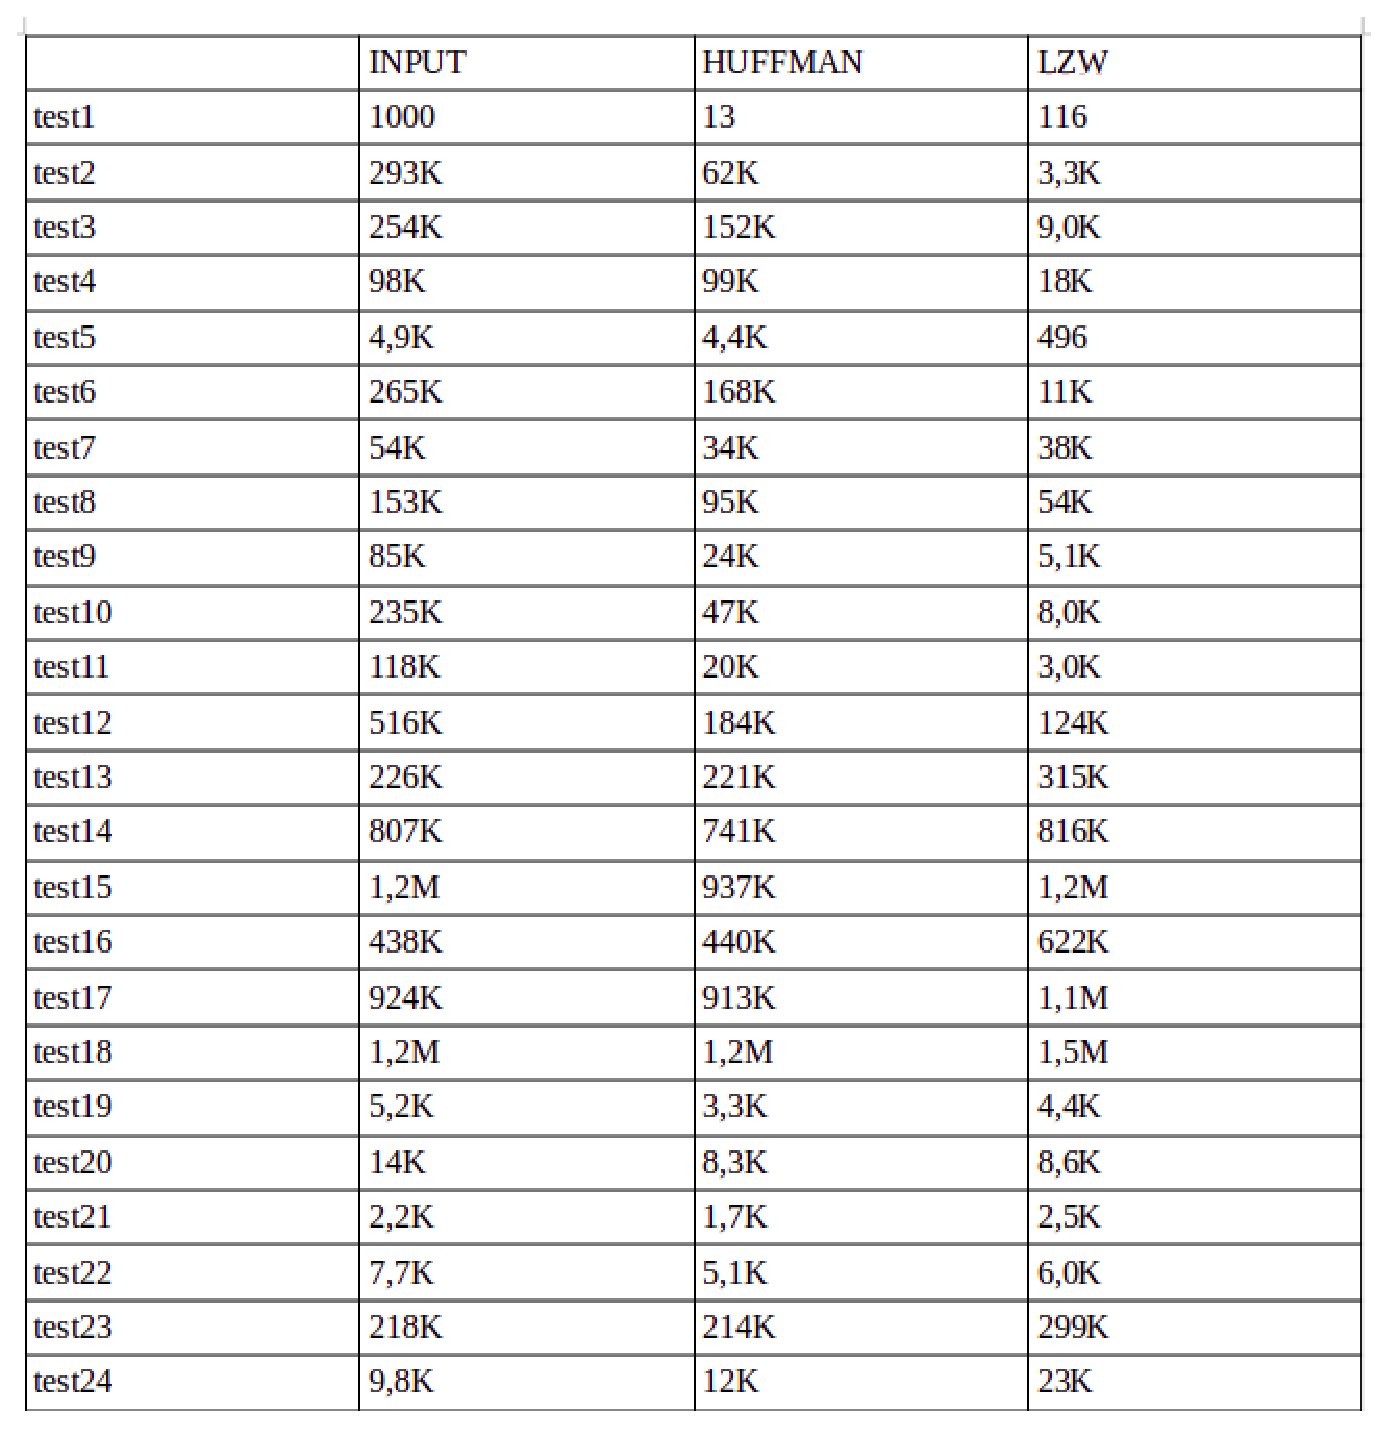
\includegraphics[width=\textwidth]{tabel3.eps}
    \caption{Tabel ce compara dimensiunea fisierului de intrare cu dimensiuniea fisierului comprimat
    rezultat in urma rularii celor doi algoritmi} \label{fig1}
    \end{figure}

In continuare am realizat o reprezentare grafica a eficientei celor 2 algoritmi in functie de testele de intrare.
Pe axa OX apare numarul testului iar pe axa OY este dat in procente
gradul de compresie rezultat (dimensiunea fisierului de iesire / dimensiunea fisierului de intrare).


\begin{figure}
\includegraphics[width=\textwidth]{tabel2.eps}
\caption{Grafic ce compara procentul de compresie al fisierelor rezultate in urma rularii celor doi algoritmi} \label{fig2}
\end{figure}

\section{Concluzii}

Din graficul reprezentat anterior se poate observa ca algoritmul LZW are o eficienta foarte buna cand vine vorba de fisiere text mari (si fisierele
bitmap ce contin putine culori), in timp ce Huffman reuseste sa realizeze o compresie mai slaba, dar in continuare relevanta pe o gama larga de fisiere de intrare
(fisierul comprimat are, in majoritatea cazurilor, o dimensiune mai mica decat cel de input, chiar daca aceasta consta doar in cativa KB).

In concluzie, algoritmul LZW ar fi eficient in practica doar pentru comprimarea fisierelor text foarte mari, caz in care dictionarul sau
ar avea ocazia de a ajunge la o dimensiune considerabila, avand deci o probabilitate foarte mare de a refolosi cuvintele deja intalinte.

In schimb, algoritmul Huffman are o probabilitate mai mare de a realiza o compresie in general eficienta pe o gama larga de fisiere cu format variat, deoarece acesta
nu are nevoie sa se ghideze dupa un standard secvential pentru a da un randament bun.

Facand o medie a rezultatelor obitnute anterior, gradul mediu de compresie al algoritmului Huffman este de 66.963\%, in timp ce pentru LZW, acesta este de 67.877\%.
Daca am alege sa ignorma ultimul test (deoarece ambii sunt ineficienti), cele doua numere ar deveni: 64.968\% pentru Huffman si 60.619\% pentru LZW, caz in care algoritmul
LZW s-ar comporta mai bine pentru gama teste alese.

Datorita acestei diferente fragile intre cei doi algoritmi, nu putem concluziona ca unul este mai bun decat celalalt, rezultatul depinzand
de datele de intrare alese.



% %%% TODO
\begin{thebibliography}{8}
\bibitem{ref_article1}
Autor, Gajendra Sharma, Analysis of Huffman Coding and Lempel-Ziv-Welch (LZW) Coding as
Data Compression Techniques\textbf{}

\bibitem{ref_url1}
\url{https://www.geeksforgeeks.org/huffman-coding-greedy-algo-3/}

\bibitem{ref_url2}
\url{https://www.programiz.com/dsa/huffman-coding}

\bibitem{ref_url3}
\url{http://www.cas.mcmaster.ca/~cs2c03/2020/LN21-2020.pdf}

\bibitem{ref_url4}
\url{https://www.youtube.com/watch?v=j2HSd3HCpDs\&t=428s}

\bibitem{ref_url5}
\url{https://www.youtube.com/watch?v=dM6us854Jk0}

\bibitem{ref_url6}
\url{https://www.youtube.com/watch?v=JsTptu56GM8}

\bibitem{ref_url7}
\url{https://www.geeksforgeeks.org/lzw-lempel-ziv-welch-compression-technique/}

\bibitem{ref_url8}
\url{https://stackoverflow.com/questions/6189765/big-o-complexities-of-algorithms-lzw-and-huffman}
\end{thebibliography}

\end{document}
